% !TEX root = main.tex

\section{极大似然与贝叶斯参数估计} % 3.1-3.5 3.7-3.8 (3.9)
% 参数估计方法
%  3.2 最大似然
%  3.3 贝叶斯
%  3.4 贝叶斯-高斯
%  3.5 贝叶斯-一般(递归)
%  3.7 维度问题
% Fisher线性判别
% 3.9 EM算法

假设样本集$\mD$中有$n$个样本$\vx_1,\ldots,\vx_n$,由于这些样本均\textbf{独立抽取},故
\[p(\mD\mid\vtheta)=\prod_{k=1}^np(\vx_k\mid\vtheta)\]
这里的$\vtheta$为参数向量。

\subsection{极大似然估计}
定义对数似然为
\[\ell(\vtheta)=\ln p(\mD\mid\vtheta)\]
进而
\[\hat{\vtheta}=\argmax_{\vtheta}\ell(\vtheta)\]
求解最大似然估计值的必要条件为
\[\nabla_{\vtheta}\ell = 0\]

高斯分布若均值和协方差矩阵均未知,则最大似然估计结果为
\[\begin{aligned}
\hat{\vmu} &= \frac{1}{n}\sum_{k=1}^n\vx_k\\
\hat{\Sigma} &= \frac{1}{n}\sum_{k=1}^n(\vx_k-\hat{\vmu})(\vx_k-\hat{\vmu})^\T\approx\E{(\vx-\hat{\vmu})(\vx-\hat{\vmu})^\T}
\end{aligned}\]
注意上述对方差的估计是有偏的估计。
\begin{figure}[H]
\centering
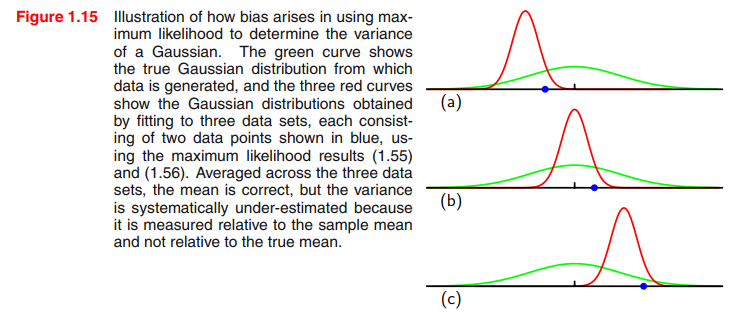
\includegraphics[width=0.8\linewidth]{fig/biased_ML_Gaussian.png}
\end{figure}

而\textbf{样本协方差矩阵}的无偏估计如下
\[C=\frac{1}{n-1}\sum_{k=1}^n(\vx_k-\hat{\vmu})(\vx_k-\hat{\vmu})^\T\]

\subsection{贝叶斯参数估计}
在最大似然估计方法中,将需要估计的参数向量$\vtheta$看作一个确定而未知的参数,而在贝叶斯方法中,我们将参数向量$\vtheta$\textbf{本身看作一个随机变量},已有的训练样本可以使我们把对于$\vtheta$的初始密度估计(先验)转为后验概率密度。

\begin{figure}[H]
\centering
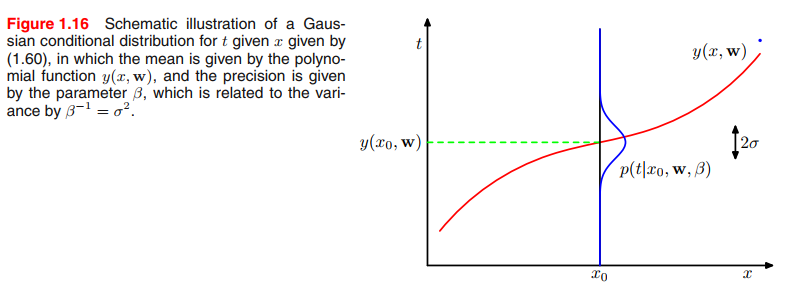
\includegraphics[width=0.8\linewidth]{fig/bayesian_est.png}
\end{figure}
% 将训练样本依据类别归到$c$个次样本集$\mD_1,\ldots,\mD_c$中,结合先验,贝叶斯公式可表成
% \[P(\omega_i\mid\vx)=\frac{p(\vx\mid\omega_i,\mD_i)P(\omega_i)}{\sum_{j=1}^cp(\vx\mid\omega_j,\mD_j)P(\omega_j)}\]

已知训练样本$\mD$,这些样本都从固定但未知的概率密度函数$p(\vx)$中独立抽取,要求根据这些样本估计$p(\vx\mid\mD)$,即贝叶斯学习的核心问题。

得到贝叶斯估计的核心公式(Gibbon)
\[\begin{aligned}
p(\vx\mid\mD)&=\int p(\vx,\vtheta\mid\mD)\diff\vtheta
=\int p(\vx\mid\vtheta,\mD)p(\vtheta\mid\mD)\diff\vtheta\\
&=\int p(\vx\mid\vtheta)p(\vtheta\mid\mD)\diff\vtheta
\end{aligned}\]
后一式成立的原因是测试样本$\vx$和训练样本集$\mD$的选取是独立进行的。
根据贝叶斯公式
\[p(\vtheta\mid\mD)=\frac{p(\mD\mid\vtheta)p(\vtheta)}{\int p(\mD\mid\vtheta)p(\vtheta)\diff\vtheta}=\alpha\prod_{k=1}^np(\vx_k\mid\vtheta)p(\vtheta)\]
其中$\alpha$是一个依赖于样本集$\mD$的归一化系数,不依赖于$\vtheta$。

当先验$p(\vtheta)$为高斯密度时,$p(\vtheta\mid\mD)$依然为正态分布,称为再生(reproducing)函数,将$p(\vtheta)$称为共轭(conjugate)先验。

考虑样本数不断增加的过程
\[p(\vtheta\mid\mD^n)=\frac{p(\vx_n\mid\vtheta)p(\vtheta\mid\mD^{n-1})}{\int p(\vx_n\mid\vtheta)p(\vtheta\mid\mD^{n-1})\diff\vtheta}\]
当没有观测样本时,$p(\vtheta\mid\mD^0)=p(\vtheta)$,反复应用上述公式有概率密度函数$p(\vtheta),p(\vtheta\mid\vx_1),p(\vtheta\mid\vx_1,\vx_2)$等,实际上即增量学习(incremental learning)。

而最大后验(maximum a posteriori, MAP)则是使$p(\mD\mid\vtheta)p(\vtheta)$取最大值的参数向量$\vtheta$,这里通常先乘起来再取对数
\[\argmax_{\vtheta} \lrp{\ln p(\mD\mid\vtheta) + \ln p(\vtheta)}
=\argmax_{\vtheta}\lrp{\sum_{k=1}^n\ln p(\vx_k\mid\vtheta)+\ln p(\vtheta)}\]

可以比较最大似然与贝叶斯之间的差异。
\begin{center}
\begin{tabular}{|c|c|c|}\hline
 & 最大似然 & 贝叶斯\\\hline
估计对象 & 单一参数 & 完整分布\\\hline
计算复杂度 & 微分 & 多重积分\\\hline
可理解性 & 确定易理解 & 不确定不易理解\\\hline
先验的准确程度 & 不准确 & 准确\\\hline
\end{tabular}
\end{center}

% \subsection{维数问题}
% 引入新的特征
% 计算复杂度
% 过拟合
% PCA

\subsection{Fisher线性判别}
PCA方法寻找的是用来有效表示的主轴方向,而判别分析方法(discriminant analysis)寻找的是用来有效\textbf{分类}的方向。

考虑将$d$维空间中的数据点投影到一条直线上,以最大限度区分各类数据点的投影方向。
假设有一组$n$个$d$维的样本$\vx_1,\ldots,\vx_n$分属两个不同类别,其中$n_1$个样本的子集$\mD_1$属于$\omega_1$,$n_2$个样本的子集$\mD_2$属于$\omega_2$。
对$\vx$中各个成分做线性组合,得到点积\footnote{回忆高中知识,点积相当于做投影,将$\vx$往直线$\vw$上投影}$y=\vw^\T\vx$,进而全部$n$个样本产生$n$个结果$y_1,\ldots,y_n$相应属于$\mY_1$和$\mY_2$。
\begin{figure}[H]
\centering
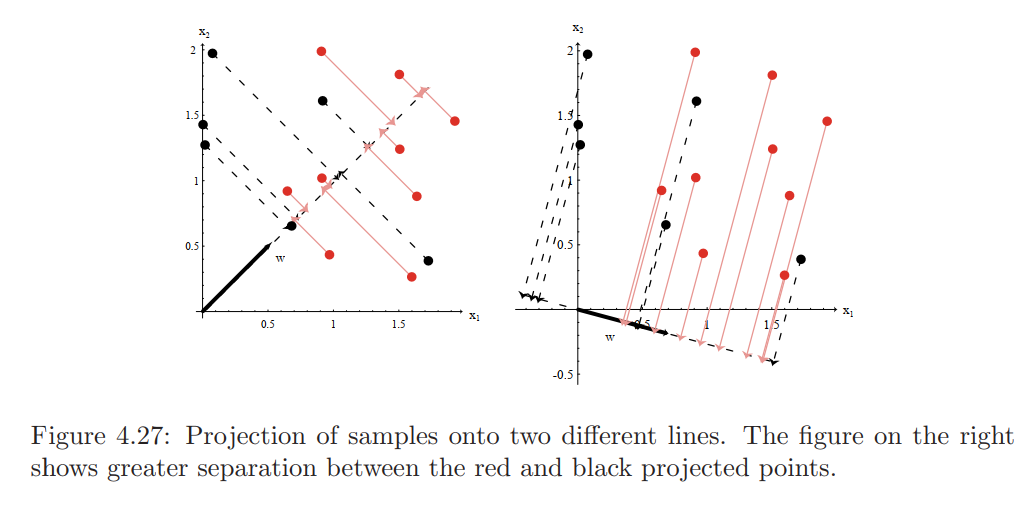
\includegraphics[width=0.8\linewidth]{fig/Fisher.png}
\end{figure}

如何确定最佳的直线方向$\vw$得到最佳的分类效果,一个衡量标准即样本均值的差。
设原样本第$i$个类别的均值为$\vm_i$,则投影后的样本均值为$\tilde{\vm}_i=\vw^\T\vm_i$。
样本均值之差为
\[|\tilde{\vm}_1-\tilde{\vm}_2|=|\vw^\T(\vm_1-\vm_2)|\]
可以通过$\vw$幅值方法来得到任意大小的均值之差,但这样子没有意义。
因此定义类别$\omega_i$的类内散布(scatter)/方差如下
\[\tilde{s}_i^2=\sum_{y\in\mY_i}(y-\tilde{m})^2\]
这样$1/n(\tilde{s}_1^2+\tilde{s}_2^2)$即为全部数据总体方差的估计,$\tilde{s}_1^2+\tilde{s}_2^2$称为投影样本的总类内散布。

故Fisher线性可分性准则要求在投影$y=\vw^\T\vx$下
\[\max_{\vw} J(\vw):=\frac{|\tilde{m}_1-\tilde{m}_2|^2}{\tilde{s}_1^2+\tilde{s}_2^2}\]
即均值差尽可能大,同时类内方差尽可能小。

定义类内散布矩阵$S_i$和总类内散布矩阵$S_W$如下
\[\begin{aligned}
S_i &= \sum_{\vx\in\mD_i}(\vx-\vm_i)(\vx-\vm_i)^\T\\
S_W &= S_1+S_2
\end{aligned}\]
可求得
\[\begin{aligned}
\tilde{s}_i^2 &= \vw^\T S_i\vw\\
\tilde{s}_1^2+\tilde{s}_2^2 &= \vw^\T S_W\vw\\
\end{aligned}\]
而投影样本均值之差
\[\begin{aligned}
S_B &= (\vm_1-\vm_2)(\vm_1-\vm_2)^\T\\
(\tilde{\vm}_1-\tilde{\vm}_2)^2 &= \vw^\T S_B\vw
\end{aligned}\]
其中$S_B$称为总类间散布矩阵。
$S_W$和$S_B$都是对称且半正定的。

进而原来的准则函数可写成
\[J(\vw)=\frac{\vw^\T S_B\vw}{\vw^\T S_W\vw}\]
称为广义瑞利商,可证令其最大化
\[S_B\vw=\lambda S_W\vw\]
一般情况下
\[\argmax_{\vw}J(\vw)=S_W^{-1}(\vm_1-\vm_2)\]